\documentclass[11pt,a4paper]{article}

\NewDocumentCommand{\nomeAluno}{}{Charles Quirino Pimenta}

\usepackage[brazil]{babel}
\usepackage[T1]{fontenc}
\usepackage[utf8]{inputenc}
\usepackage{lmodern}
\usepackage{ae}
\usepackage{xargs}
\usepackage{indentfirst}
\usepackage[margin=2cm]{geometry}
\usepackage{amsthm,amssymb,amsfonts,amsmath}
\usepackage{psfrag}
\usepackage{booktabs}
\usepackage{colortbl,booktabs}
\usepackage{enumerate}
\usepackage[shortlabels]{enumitem}
\usepackage{csquotes}
\usepackage{multicol}
% Para plotar tabelas
\usepackage{booktabs}
\usepackage{array}
\usepackage{colortbl}
\usepackage{booktabs}
\usepackage{array}
\usepackage{placeins}
\usepackage{
tikz,
relsize,
amsmath,
booktabs,
tikz
}
\usepackage{caption}
\usepackage{subcaption}
\usepackage{graphicx}
\usepackage{float}
\usepackage[framemethod=tikz]{mdframed}
 

\begin{document}
\thispagestyle{empty}

\noindent
\begin{minipage}{0.8\linewidth}
  {\Large\bf Universidade Federal de Minas Gerais}\\
  {\small ESCOLA DE ENGENHARIA}\\
  {\sc Departamento de Engenharia Elétrica}
\end{minipage} 
\hfill 
\begin{minipage}{3cm}
  
\includegraphics[width=3cm]{ufmg_ext.pdf}
\end{minipage}

\vspace{1mm}

\noindent
\hrule

\vspace{2.0cm}

\vfill

\begin{center}
  \Large \textsc{\textbf{Trabalho I}}\\ 
  \Large \textsc{\textbf{Controle Usando Sistemas Nebulosos}}
\end{center}

\vfill

\begin{center}
  \Large\textsc{\textbf{Robô Móvel}}
\end{center}

\vfill

\begin{flushright}
\begin{minipage}{12.0cm}
{\bf Aluno:} \nomeAluno \\
\end{minipage}
\end{flushright}

\vfill

\begin{center}
  \today
\end{center}

\vfill

\newpage 
\graphicspath{ {./imagens/} }

\section{Descrição do Problema}
Considere o modelo cinemático de um uniciclo, dado por:
    \begin{align*}
            \dot{x} &= v_t cos(\theta)\\
            \dot{y} &= v_t sin(\theta)\\
            \dot{\theta} &= \omega
    \end{align*}

Em que $x$, $y$ e $\theta$ representam a posição em x, posição em y e orientação do veículo, enquanto
que $v_t$ e $\omega$representam as velocidades de translação e angular do veículo.

\section{Descrição da solução proposta}

Este trabalho propõe uma forma de se controlar o sistema para que ele siga uma referência de posição desejada utilizando linguagem natural. O controlador implementado foi baseado na técnica de controladores fuzzy utilizando o método de inferência por regras de Mamdani. 

A referência utilizada é um outro carrinho hipotético que pode ser controlado manualmente ou programado para realizar certos movimentos pré-definidos dentro de uma área especifica. O ambiente de simulação foi provido pelo professor no ambiente moodle e abaixo pode-se observar uma figura que demonstra a aparência do simulador utilizado. O carrinho bege é a nossa referência enquanto o carrinho amarelo é o nosso carrinho a ser controlado.

\begin{figure}[H] 
    \centering
    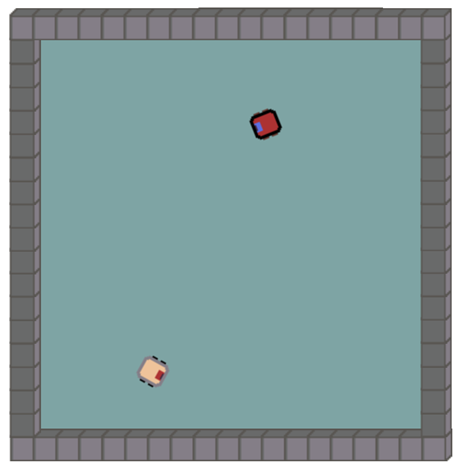
\includegraphics[scale=0.5]{carrinho_base.png}
    \caption{Ambiente de simulação}
\end{figure}
 
Inicialmente, para o projeto do controlador, identificou-se as entradas e saídas do controlador. As entradas são o erro do ângulo em relação a referência (e$\theta$) e o erro de posição do carrinho (Exy). A representação geométrica das entradas utilizadas é exibida na figura a seguir.

\begin{figure}[H] 
    \centering
    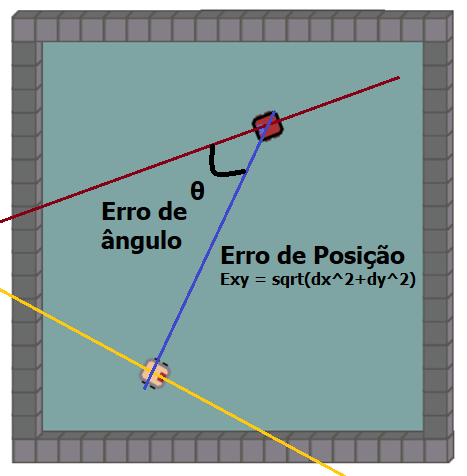
\includegraphics[scale=0.5]{imagens/carrinho_erros.png}
    \caption{Ambiente de simulação}
\end{figure}

Onde o Onde $\theta$, nesta figura, representa o ângulo atual de inclinação em relação a normal do corpo do carrinho de referência. O erro de posição é a distancia euclidiana no plano cartesiano entre ambos os carrinhos.

As saídas do sistema são a Velocidade Angular e a Velocidade Linear. A primeira saída será aplicada para causar uma rotação do carrinho controlado sobre seu próprio eixo em um intervalo de $[-\pi,+\pi]$ fazendo com que o carrinho gire em sentido horário ou anti horário. A segunda saída fará o carrinho deslocar-se sobre o vetor de direção em que estiver apontando com velocidades em um intervalo de $[-V_{max},+V_{max}]$ . 

\section{Projeto do controlador fuzzy do carrinho}
    \subsection{Variáveis Linguísticas}
        \begin{itemize}
            \item{\bf{Antecedentes}}
                \begin{itemize}
                    \item Erro de ângulo
                    \item Erro de posição
                \end{itemize}
            \item{\bf{Saídas}}
                \begin{itemize}
                        \item Velocidade angular
                        \item Velocidade
                \end{itemize}
        \end{itemize}
    \subsection{Funções de pertinência}
    \begin{itemize}
        \item{\bf{Erro de ângulo}}
            \begin{itemize}
                \item Universo de discurso: $[-\pi,\pi]$
                \item Formato das funções de pertinência: Trapezoidal
                \item Número de conjuntos nebulosos: 5
            \end{itemize}  
            
            \begin{table}[H]
                \centering
                \begin{tabular}{|c|c|c|c|c|}
                    \hline
                    Conjunto                         & Esq   & C\_Esq & C\_Dir & Dir \\ \hline
                    Erro de Ângulo Negativo Grande   & -5    & -5    & -2.5  & -2    \\
                    Erro de Ângulo Negativo Pequeno  & -3    & -2    & -1    & 0     \\
                    Erro de Ângulo Nulo              & -1    & -0.5  & 0.5   & 1     \\
                    Erro de Ângulo Positivo Pequeno  & 0     & 1     & 2     & 3     \\
                    Erro de Ângulo Positivo Grande   & 2     & 2.5   & 5     & 5     \\ \hline
                \end{tabular}
                \caption{Erro de ângulo}
            \end{table}

            \begin{figure}[H] 
                \centering
                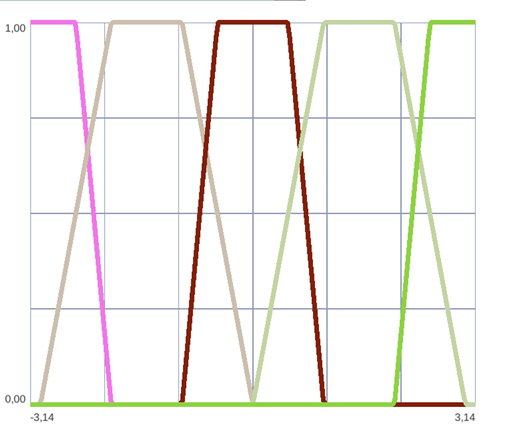
\includegraphics[scale=0.5]{in_angulo.png}
                \caption{Erro de ângulo}
            \end{figure}
        
        \item{\bf{Erro de posição}}
            \begin{itemize}
                \item Universo de discurso: $[-10,10]$
                \item Formato das funções de pertinência: Trapezoidal
                \item Número de conjuntos nebulosos: 5
            \end{itemize}

            \begin{table}[H]
                \centering
                \begin{tabular}{|c|c|c|c|c|}
                    \hline
                    Conjunto                         & Esq & C\_Esq & C\_Dir & Dir \\ \hline
                    Erro de Posição Negativo Grande  & -10 & -10    & -2.5   & -2  \\
                    Erro de Posição Negativo Pequeno & -3  & -2     & -1     & 0   \\
                    Erro de Posição Nulo             & -1  & -0.5   & 0.5    & 1   \\
                    Erro de Posição Positivo Pequeno & 0   & 1      & 2      & 3   \\
                    Erro de Posição Positivo Grande  & 2   & 2.5    & 10     & 10  \\ \hline
                \end{tabular}
                \caption{Erro de posição}
            \end{table}

            \begin{figure}[H] 
                \centering
                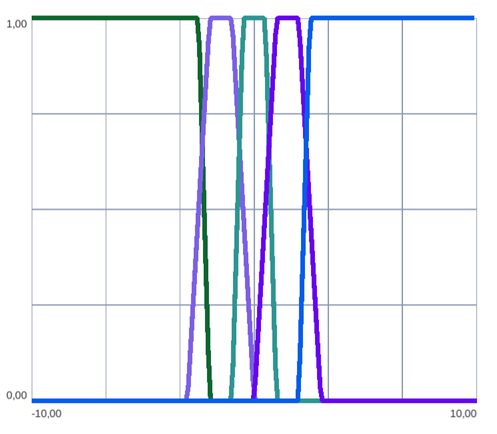
\includegraphics[scale=0.5]{imagens/in_posicao.png}
                \caption{Erro de posição}
            \end{figure}
            
        \item{\bf{Velocidade angular}}
            \begin{itemize}
                \item Universo de discurso: $[-5,5]$
                \item Formato das funções de pertinência: Trapezoidal
                \item Número de conjuntos nebulosos: 5
            \end{itemize}

            \begin{table}[H]
                \centering
                \begin{tabular}{|c|c|c|c|c|}
                    \hline
                    Conjunto               & Esq & C\_Esq & C\_Dir & Dir \\ \hline
                    Gira Rápido a Esquerda & -5  & -5     & -2.5   & -2  \\
                    Gira Lento a Esquerda  & -3  & -2     & -1     & 0   \\
                    Não Gira               & -1  & -0.5   & 0.5    & 1   \\
                    Gira Lento a Direita   & 0   & 1      & 2      & 3   \\
                    Erro Rápido a Direita  & 2   & 2.5    & 5      & 5   \\ \hline
                \end{tabular}
                \caption{Velocidade angular}
            \end{table}

            \begin{figure}[H] 
                \centering
                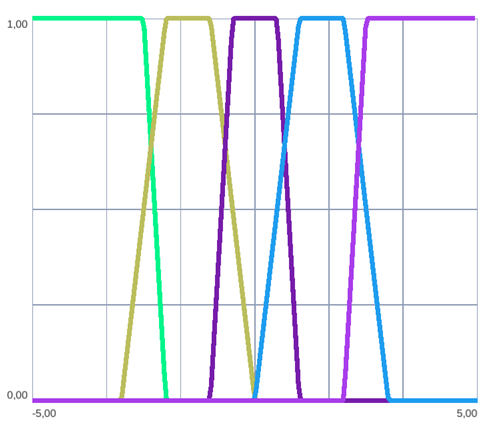
\includegraphics[scale=0.5]{imagens/out_velocidadeang.png}
                \caption{Velocidade angular}
            \end{figure}
            
        \item{\bf{Velocidade}}
            \begin{itemize}
                \item Universo de discurso: $[-5,5]$
                \item Formato das funções de pertinência: Trapezoidal
                \item Número de conjuntos nebulosos: 5
            \end{itemize}

            \begin{table}[H]
                \centering
                \begin{tabular}{|c|c|c|c|c|}
                    \hline
                    Conjunto               & Esq   & C\_Esq & C\_Dir & Dir   \\ \hline
                    Freia Muito            & -5    & -5     & -2.5   & -2    \\
                    Freia Pouco            & -3    & -2     & -1     & 0     \\
                    Nem Acelera e Nem Freia   & -1    & -0.5   & 0.5    & 1     \\
                    Acelera Pouco          & 0     & 1      & 2      & 3     \\
                    Acelera Muito          & 2     & 2.5    & 5      & 5     \\ \hline
                \end{tabular}
                \caption{Velocidade}
            \end{table}

            \begin{figure}[H] 
                \centering
                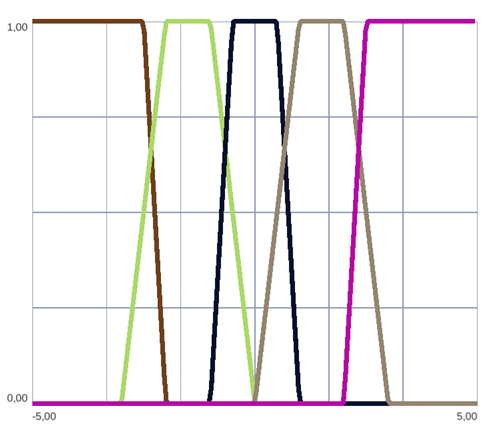
\includegraphics[scale=0.5]{imagens/out_velocidade.png}
                \caption{Velocidade}
            \end{figure}

    \end{itemize}
    \subsection{Banco de regras}
        Implementou-se o método de inferência por regras de Mamdani. Portanto, foram definidas 25 regras que descrevem como o controlador funciona. Todas as regras encontram-se descritas na lista a seguir. 
        Entretanto, após implementação e simulação, observou-se que uma regra extra foi inserida por engano. No caso a Regra 17, que encontra-se em destaque, entra em conflito com a Regra 18.

        \begin{enumerate}[{\textbf{Regra}} 1 {\textbf{:}} ]
            \item Se Erro de Ângulo Nulo e Erro de Posição Nulo, então Não Gira e Nem Acelera e Nem Freia
            \item Se Erro de Ângulo Nulo e Erro de Posição Negativo Pequeno, então Não Gira e Freia Pouco
            \item Se Erro de Ângulo Nulo e Erro de Posição Positivo Pequeno, então Não Gira e Acelera Pouco
            \item Se Erro de Ângulo Nulo e Erro de Posição Negativo Grande, então Não Gira e Freia Muito
            \item Se Erro de Ângulo Nulo e Erro de Posição Positivo Grande, então Não Gira e Acelera Muito
            \item Se Erro de Ângulo Negativo Pequeno e Erro de Posição Nulo, então Gira Lento a Esquerda e Nem Acelera e Nem Freia
            \item Se Erro de Ângulo Negativo Pequeno e Erro de Posição Negativo Pequeno, então Gira Lento a Esquerda e Freia Pouco
            \item Se Erro de Ângulo Negativo Pequeno e Erro de Posição Negativo Grande, então Gira Lento a Esquerda e Freia Muito
            \item Se Erro de Ângulo Negativo Pequeno e Erro de Posição Positivo Pequeno, então Gira Lento a Esquerda e Acelera Pouco
            \item Se Erro de Ângulo Negativo Pequeno e Erro de Posição Positivo Grande, então Gira Lento a Esquerda e Acelera Muito
            \item Se Erro de Ângulo Negativo Grande e Erro de Posição Nulo, então Gira Rápido a Esquerda e Nem Acelera e Nem Freia
            \item Se Erro de Ângulo Negativo Grande e Erro de Posição Negativo Pequeno, então Gira Rápido a Esquerda e Freia Pouco
            \item Se Erro de Ângulo Negativo Grande e Erro de Posição Negativo Grande, então Gira Rápido a Esquerda e Freia Muito
            \item Se Erro de Ângulo Negativo Grande e Erro de Posição Positivo Pequeno, então Gira Rápido a Esquerda e Acelera Pouco
            \item Se Erro de Ângulo Negativo Grande e Erro de Posição Positivo Grande, então Gira Rápido a Esquerda e Acelera Muito
            \item Se Erro de Ângulo Positivo Pequeno e Erro de Posição Nulo, então Gira Lento a Direita e Nem Acelera e Nem Freia
            \item\begin{mdframed}[hidealllines=true,backgroundcolor=blue!20]
            Se Erro de Ângulo Positivo Pequeno e Erro de Posição Negativo Pequeno, então Gira Lento a Direita e Nem Acelera e Nem Freia
            \end{mdframed}
            \item Se Erro de Ângulo Positivo Pequeno e Erro de Posição Negativo Pequeno, então Gira Lento a Direita e Freia Pouco
            \item Se Erro de Ângulo Positivo Pequeno e Erro de Posição Negativo Grande, então Gira Lento a Direita e Freia Muito
            \item Se Erro de Ângulo Positivo Pequeno e Erro de Posição Positivo Pequeno, então Gira Lento a Direita e Acelera Pouco
            \item Se Erro de Ângulo Positivo Pequeno e Erro de Posição Positivo Grande, então Gira Lento a Direita e Acelera Muito
            \item Se Erro de Ângulo Positivo Grande e Erro de Posição Nulo, então Erro Rápido a Direita e Nem Acelera e Nem Freia
            \item Se Erro de Ângulo Positivo Grande e Erro de Posição Negativo Pequeno, então Erro Rápido a Direita e Freia Pouco
            \item Se Erro de Ângulo Positivo Grande e Erro de Posição Negativo Grande, então Erro Rápido a Direita e Freia Muito
            \item Se Erro de Ângulo Positivo Grande e Erro de Posição Positivo Pequeno, então Erro Rápido a Direita e Acelera Pouco
            \item Se Erro de Ângulo Positivo Grande e Erro de Posição Positivo Grande, então Erro Rápido a Direita e Acelera Muito

        \end{enumerate}

        \subsection{Definições dos operadores implicação e defuzzificador}
            \begin{description}
                \item [S-norma Soma de Einstein] Os operadores de união nebulosa normalmente recebem o nome de s-normas. Para este projeto desejava-se um comportamento com transição suave das ações de controle. Por este motivo utilizou-se a soma de Einstein como operador de união nebulosa. A operação soma de Einstein é definida como:
    
                \begin{equation*}
                    S_{e_s}(a,b)=\frac{a+b}{1+ab}
                \end{equation*}
    
                \item [T-norma Produto] Os operadores de interseção nebulosa normalmente recebem o nome de t-normas. Para este projeto desejava-se um comportamento com transição suave das ações de controle. Por este motivo utilizou-se o Produto Algébrico como operador de interseção nebulosa. A operação Produto Algébrico é definido como:
    
                \begin{equation*}
                    t_p(a,b)=ab
                \end{equation*}
                
                \item [Implicação do Produto (Mandani)] neste tipo de inferência, utiliza-se: 
                    \begin{itemize}
                        \item [i.] inferência individual de cada regra com combinação pela união
                        \item [ii.] Implicação do produto de Mamdani
                        \item [iii.] produto algébrico para todas as t-normas e max para todas as s-normas.
                    \end{itemize}
    
                    \begin{equation*}
                        \mu_{\tilde{B}_k}(y)=  \max\limits_{k=1\hdots r} \left( \sup\limits_{ x \in \mathcal{U}} \left( \mu_{\tilde{A}}(x)\left( \prod_{i=1}^{n} \mu_{A^k_i}(x_i)  \right) \mu_{B^k}(y)\right) \right)
                    \end{equation*}
                    
                \item [Fuzzificação Singleton] Para a operação de Fuzzificação Singleton, gera-se um conjunto nebuloso que corresponde somente àquele ponto, ou seja:
                \begin{equation*}
                    \mu_{\tilde{A}}(a,b)=
                     \begin{cases}
                        1, & \text{se \textbf{$x=x^{\star}$}}\\
                        0, & \text{caso contrário}
                    \end{cases}      
                \end{equation*}
                \item [Defuzzificação Média dos Máximos (MoM)] Para a operação de defuzzificação Média dos Máximos, Os valores relativos ao máximo da função são selecionados e é tomada a sua média aritmética.
                \begin{equation*}
                    y^{\star}= \frac{\sum_{k=1}^{r} max(\mu_{\tilde{B}_k}(y))}{r}\\
                \end{equation*}
            \end{description}

\section{Resultados e discussão}

    \subsection{Simulação com referência Manual}

    \subsection{Simulação com referência Retangular}

    \subsection{Simulação com referência Circular} 
\end{document}